\section{Diseño e Implementación de la Arquitectura Híbrida}
\label{sec:arquitectura}

Este capítulo detalla la aportación técnica central de este TFM: la integración de Transformers y GRU en un único modelo funcional, así como la estrategia de curación de datos y la configuración del entrenamiento desde cero, con comparativa técnica frente al estado del arte.

\subsection{Arquitectura del Modelo: Hybrid Transformer-GRU}

El modelo \texttt{tfm-slm} sigue el paradigma \textbf{decoder-only} con atención causal: no existe encoder ni cross-attention, y cada token solo puede atender a posiciones anteriores. Cada uno de los 12 bloques del modelo fusiona un componente recurrente (GRU) y uno atencional (MHA) dentro del mismo bloque decoder. El proceso iterativo de desarrollo que llevó a este diseño, incluyendo las limitaciones del diseño inicial y las mejoras aplicadas, se documenta en el Capítulo~\ref{sec:implementation}.

\begin{figure}[H]
    \centering
    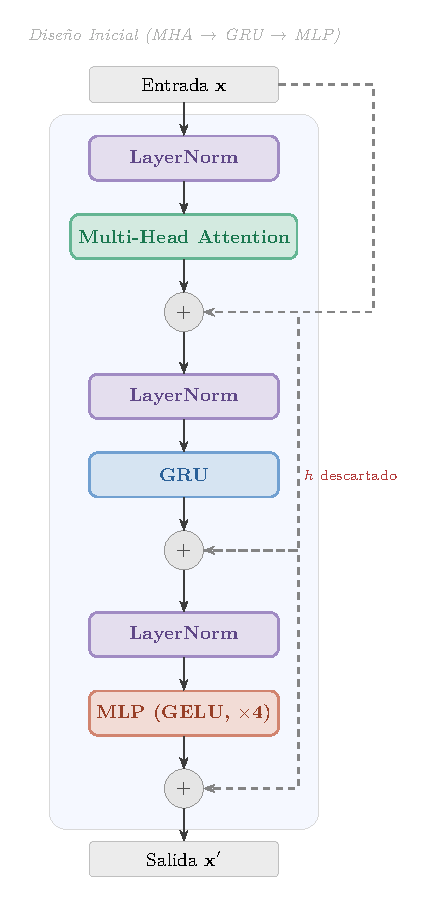
\includegraphics[width=0.45\textwidth]{images/diagrams_hybridblock/block_inicial.pdf}
    \caption{Diseño inicial del bloque híbrido (MHA $\to$ GRU $\to$ MLP). El GRU recibe una representación ya transformada por la atención, generando redundancia entre ambos componentes. El estado oculto del GRU se descartaba al final de cada bloque.}
    \label{fig:block_inicial}
\end{figure}

\begin{figure}[H]
    \centering
    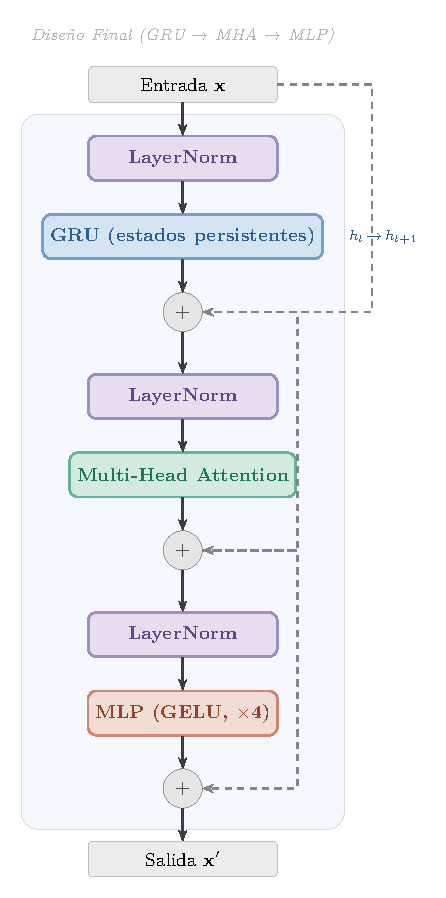
\includegraphics[width=0.45\textwidth]{images/diagrams_hybridblock/block_final.pdf}
    \caption{Diseño final del bloque híbrido (GRU $\to$ MHA $\to$ MLP). El GRU procesa la entrada bruta y propaga su estado oculto al bloque siguiente ($h_l \to h_{l+1}$), dotando al modelo de memoria vertical a través de la profundidad de la red.}
    \label{fig:block_final}
\end{figure}

\begin{figure}[H]
    \centering
    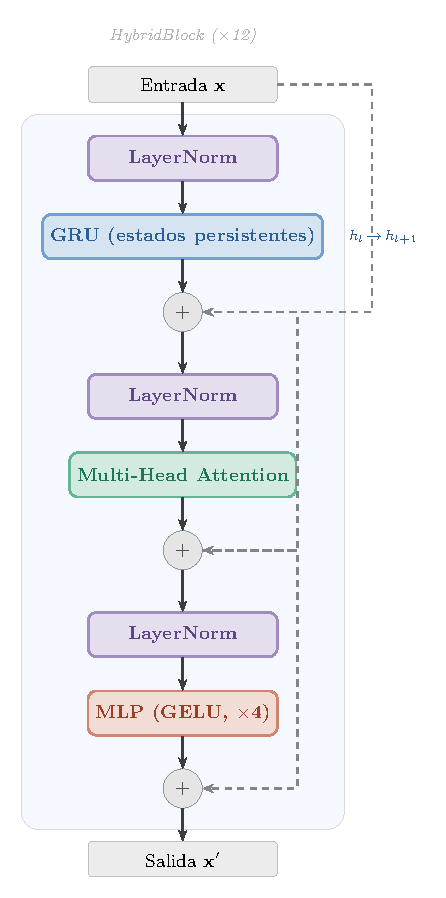
\includegraphics[width=0.55\textwidth]{images/diagrams_hybridblock/hybridblock.pdf}
    \caption{HybridBlock: integración de GRU y MHA en un único bloque. Cada sub-componente aplica Pre-LayerNorm y conexión residual. El estado oculto del GRU ($h_l \rightarrow h_{l+1}$) persiste entre bloques consecutivos, dotando al modelo de memoria vertical a lo largo de la profundidad de la red.}
    \label{fig:hybridblock}
\end{figure}

\begin{figure}[H]
    \centering
    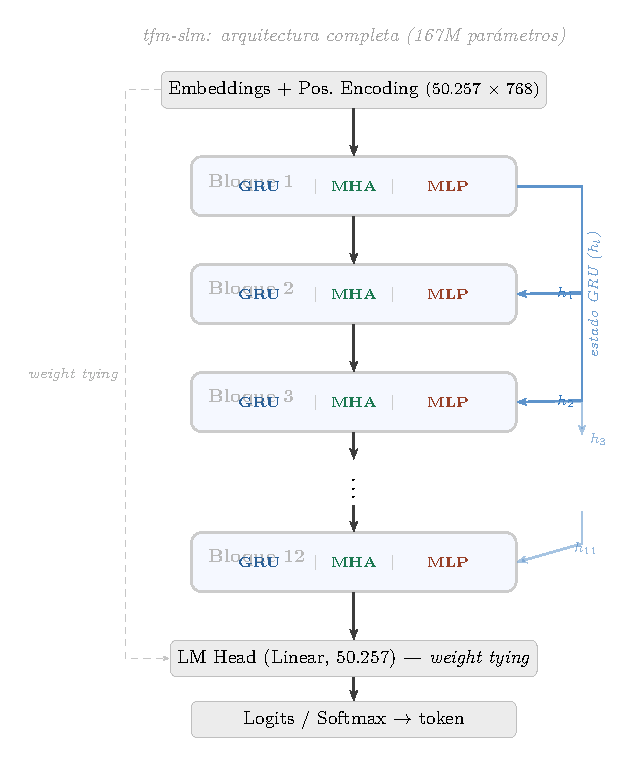
\includegraphics[width=0.58\textwidth]{images/diagrams_hybridblock/model_stack.pdf}
    \caption{Arquitectura completa del tfm-slm: 12 HybridBlocks apilados con flujo de activaciones (flechas negras) y canal de estados ocultos GRU (flechas azules). Cada bloque $l$ genera un estado $h_l$ que se propaga como entrada recurrente al bloque $l+1$, creando memoria vertical a través de la profundidad de la red. La capa de embeddings y el LM Head comparten pesos (\textit{weight tying}).}
    \label{fig:model_stack}
\end{figure}

\subsubsection{Especificaciones Técnicas y Parámetros}
El modelo se ha dimensionado para ser competitivo en el rango de los Small Language Models, optimizando el ancho de banda de la arquitectura para hardware de 24 GB de VRAM. A continuación se detallan las especificaciones y una comparativa directa con el modelo de referencia en la industria, SmolLM2-135M.

\paragraph{Justificación del Tokenizer:} Para esta arquitectura se ha seleccionado el tokenizer de \textbf{GPT-2} (50,257 tokens). Esta elección es estratégica por tres motivos:
\begin{enumerate}
    \item \textbf{Eficiencia de Parámetros:} Al mantener un vocabulario moderado, se minimiza el \textit{overhead} de memoria en la capa de \textit{embeddings} (38M de parámetros), permitiendo dedicar una mayor fracción de la capacidad computacional a los bloques híbridos Transformer-GRU.
    \item \textbf{Robustez Byte-level BPE:} El uso de codificación por pares de bytes (\textit{Byte-Pair Encoding}) garantiza que el modelo pueda procesar cualquier secuencia de caracteres sin generar tokens desconocidos (\textit{out-of-vocabulary}), algo crítico en la mezcla de datos técnicos y código Python.
    \item \textbf{Estandarización:} Facilita la comparabilidad directa con otros modelos de la literatura técnica, asegurando que las métricas de rendimiento dependan de la arquitectura y no de variaciones en la tokenización.
\end{enumerate}

\begin{table}[H]
\centering
\begin{tabularx}{\textwidth}{|X|c|c|}
\hline
\textbf{Especificación} & \textbf{SmolLM2-135M} & \textbf{tfm-slm (Propuesto)} \\ \hline
Arquitectura & Pure Transformer (Llama) & Hybrid Transformer-GRU \\ \hline
Parámetros Totales & ~135M & \textbf{~167M} \\ \hline
Capas (Blocks) & 30 & 12 \\ \hline
Hidden Size ($d_{model}$) & 576 & 768 \\ \hline
MLP Intermediate Size & 1536 & 3072 \\ \hline
Atención & GQA (9/3 heads) & MHA (12 heads) \\ \hline
Escalado de Memoria & Cuadrático $O(L^2)$ & \textbf{Híbrido (Linear-assisted)} \\ \hline
\end{tabularx}
\caption{Comparativa arquitectónica: tfm-slm vs. SmolLM2-135M.}
\label{tab:comparativa_smollm}
\end{table}

\begin{itemize}
    \item \textbf{Capas:} 12 bloques híbridos. Aunque posee menos capas que SmolLM2, la densidad de información por bloque es superior gracias al componente GRU.
    \item \textbf{Dimensión del Modelo ($d_{model}$):} 768.
    \item \textbf{Contexto Máximo:} 1024 tokens.
    \item \textbf{Vocabulario:} 50,257 tokens (GPT-2 Tokenizer).
    \item \textbf{Weight Tying:} Se ha implementado el amarre de pesos entre la capa de \textit{embeddings} y la cabeza de salida (\textit{LM Head}), reduciendo el uso de memoria en un 18\%.
\end{itemize}

